\documentclass [10pt, twoside, slovak, a4paper] {article}

\usepackage[slovak]{babel}
\usepackage[IL2]{fontenc}
\usepackage[utf8]{inputenc}
\usepackage{graphicx}
\usepackage{url}
\usepackage{hyperref}
\usepackage{cite}

\pagestyle{headings}

\title{Role Playing Games - RPG\thanks{Semestrálny projekt v predmete Metódy inžinierskej práce, ak. rok 2022/23, vedenie: Mgr. Martin Sabo, PhD.}}

\author{Paolo Ruggeri\\[2pt]
	{\small Slovenská technická univerzita v Bratislave}\\
	{\small Fakulta informatiky a informačných technológií}\\
	{\small \texttt{xruggeri@stuba.sk}}
	}

\date {\small 2. november 2022}

\begin{document}
\maketitle

\begin{abstract}
Role-Playing Games, skrátene RPG, je jeden z najpopularnejších a tiež jeden z najstarších herných žanrov. 
Je to žáner ktorý sa zameriava na sýstem hrania rôzných tried, napríklad nejakeho hrdinu alebo čarodejníka, tiež obsahuje systém stavby a zlepšenia vlastnej postavy.
Tento článok sa bude zameriavať na hístoriu tohto žanru, druhý RPG, aké su hlavné systémy a charakteristiky použité v týchto hrach, ktoré hry ovplyvnili tento žáner, a tiež nejake výsoko ocenene hry.
\end {abstract}

\section{Hístoria}

Role-Playing Games začali ako žáner stolových hier, ako napríklad Dungeon and Dragons. V DnD si hráči vymyslia postavu, a jeden hráč ma rolu rozprávača, alebo Gamemaster, ktorý rozpráva príbeh a rozhoduje aké zápletky budú. Táto stolová hra sa stala veľkou inšpiráciou pre mnoho prvých RPG videohier.

Jedny z prvých RPG videohier sú Wizardry a Ultima, v 1980. Tieto hry boli postavené na textovom formáte s ASCII grafikou. V týchto hrách sa vytvorila šablóna ktorá väčšina RPG dodnes ešte používa: Viacero rol a tried pre postavu; vymeniteľne vybavenie a zlepšovanie postavy; Turn-Based Combat riadené s menu; veľký dôraz na rozvoj príbehu. V roku 1980 tiež vyšla veľmi významná hra pre tento žáner, Rouge. Používala ASCII grafiku pre náhodné generovanie miest a vybavenia. Táto hrá potom vytvorila cely podžáner, rougelikes.

Prvá RPG hrá ktorá vyšla na hernej konzole bola na Atari 2600, ale RPG ako žáner si našlo svoje miesto na 8-bitovej konzole, Nintendo Entertainement System, skrátene NES. Tú vzniklo mnoho RPG ktoré sú populárne aj dodnes, napríklad Dragon Quest od Exix v 1986 alebo Final Fantasy od Square v roku 1987. Tieto hry sa tiež stali veľkou inšpiráciou pre mnohé RPG v budúcnosti. RPG na NES sa odlišovali od ďalších hrách na konzole, ako Super Mario Bros., ktoré trvali aspoň 2  hodiny aby na ukončenie hry, ale RPG mohli trvať aj viac než 24 hodín. Väčšina RPG v tomto čase boli tvorené od japonských tvorcov, s tým sa vyvinuli ich vlastné trópy a štýl rozprávania príbehu, preto sa väčšina týchto hier dáva pod žánrom JRPG, Japanese Role Playing Games. 
RPG žáner sa stál ešte viac populárnym v 16-bitovej ére, hlavne na Super Nintendo Entertainment System, skrátene SNES, s hrami ako boli Final Fantasy IV až VI, Chrono Trigger a Earthbound. 
Od zavedenia optického disku na konzolách, hlavné na Sony Playstation, RPG začali byť väčšie, mali väčší svet, viac questov, CGI scény ktoré rozvíjali príbeh viac cinematicky. Hlavná hrá ktorý ma dôraz v tomto období bola Final Fantasy VII v roku 1997, ktorá dodnes je považovaná sa jedná z najlepších hier ktoré boli vydané.


\section{Charakteristiky RPG}
\subsection {Príbeh}
Príbeh je dôležitá časť tohto žánru. Zvyčajne tieto príbehy patria do fantasy alebo sci-fi žánra. Príbeh by mal byť pútavý, tak aby hráč chcel pokračovať a skončiť tu hru. Príbeh môže byť dynamicky, rozvetvený, kde hráč vyberá medzi možnosťami a tak pokračuje príbeh, ale môže byť aj lineárny. Cez príbeh hráč chodí a skúma fiktívny svet v tejto hre, rozpráva sa s rožnými NPC a dostáva questi, to sú úlohy ktoré hráč dostáva ktoré po skončení umožňuje pokračovať hlavný príbeh alebo dostať nejakú odmenu.
\subsection{Mechaniky a Turn Based Combat}
Turn-Based Combat, alebo ťahový boj, je mechanika ktorá sa často nachádza v RPG hrách. Je to mechanika kde hráč vyberá medzi možnosťami, čo ma postava spraviť v boji, to môže byť útok na nepriateľa, použije nejaký skill alebo item, alebo utečie z boja. Výhody tohto mechanizmu je to že hrá umožňuje hráčom rozmýšľať nad najlepšou taktikou bez ohľadu na čas. Toto nie je jediný mechanizmus boja ktoré RPG hry môžu mať. Novšie hry obsahujú tiež Real-Time Combat, to je boj v reálnom čase. Zvyčajne je to v Action RPG hrách, a boj je podobný viac na akčných hrach.



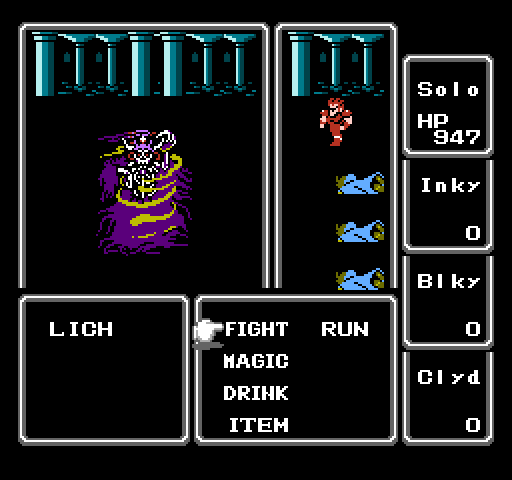
\includegraphics[scale=0.3]{FFTBC.png}


RPG hry používajú systém zlepšovania vlastnej postavy v hre. Keď hráč začne hru, tak zvyčajne postava je Level 1, začiatočná úroveň. Aby hráč mohol zlepšiť svoju postavu tak musí nazbierať požadované množstvo Experience Points, skrátene EXP. Tento systém nemusí využívať každá hra, ale veľmi často obsahujú inventár kde hráč počas hry vie nazbierať rôzne vybavenie ktoré môže zlepšiť vlastnú postavu, tieto môže hráč dostať cez skončenia questov, skúmanie sveta alebo kúpiť v hre za fiktívnu menu.


\section {podžánre RPG}
\subsection {Rougelikes}
Roguelike je žáner ktorý je ovplyvnený od hry Rogue z roku 1980. V týchto hrach zámer je objavovanie náhodne generovaného prostredia a získavanie vybavenia. Jeden z hlavných znakov tohto žánru je "permadeath", to je keď postava v hre zomrie, hra sa skonči, a treba začať od začiatku. Nejaké hry ktoré ovplyvnili tento žáner sú Hack, NetHack a Moira. V roku 1997 vyšla prvá hra z vysoko uznanej a populárnej serie Diablo od Blizzard.
\subsection{Action RPG}
Žáner RPG ktorý ma dôraz na boj v reálnom čase, namiesto klasického Turn-Based Combat, ale tiež majú veľký doraz na postavenie a zlepšovanie postavy. Tieto hry zvyčajne používajú systém boju z akčných hier, ako Hack and Slash alebo aj striekačky. Populárne hry ktoré patria do tohto žánru sú napríklad Legend of Zelda, Assassins Creed, Mass Effect a Deus Ex.
\subsection{MMO RPG}
Massively Multiplayer Online RPG, je žáner ktorý je podobný ako Action RPG, ale zameriava sa viac na multiplayer aspekt, ako socializovanie s tisíckami hráčov ktorých hrajú v tom istom svete. Hlavná vec v týchto hrach je to že tým že je to online hra, dostáva neustále aktualizácie a rozšírenie obsahu, ktorá udrží hráčov. Hry ktoré patria do tohto žánru sú napríklad RuneScape, EverQuest, World of Warcraft alebo aj Final Fantasy XIV.
\subsection{Sandbox RPG}
Sandbox RPG sú podobne ako Action RPG ale ich zámer je veľký svet s voľným pohybom. Tieto hry majú veľký počet obsahu okolo ich sveta ktoré nie sú úplne dôležite k hlavnému príbehu hry ale rozvíjajú a budujú ten fiktívny svet. Niektoré hry ktoré patria pod týmto žánrom sú Legend of Zelda Breath of the Wild, The Elder Scrolls, Xenoblade Chronicles a Dark Souls.
\subsection{Tactical RPG}
Tactitcal RPG, niekedy uznane aj za Strategy RPG, je žáner ktorý spája elementy RPG ako je budovanie postav a rozvoj príbehu s elementami strategických hier ako je hranie na izometrickej mriežke. Príklad populárnej hry ktorá patri pod týmto žánrom je X-COM.


\section {Ovplyvňujúce a vysoko uznane hry}

\nocite{*}
\bibliography{zdroje}
\bibliographystyle{alpha}

\end{document}
